\chapter{Introducción específica} % Main chapter title

\label{Chapter2}

\section{Arquitectura del dispositivo bajo prueba}
\label{sec:dut}

\begin{figure}[htbp]
	\centering
	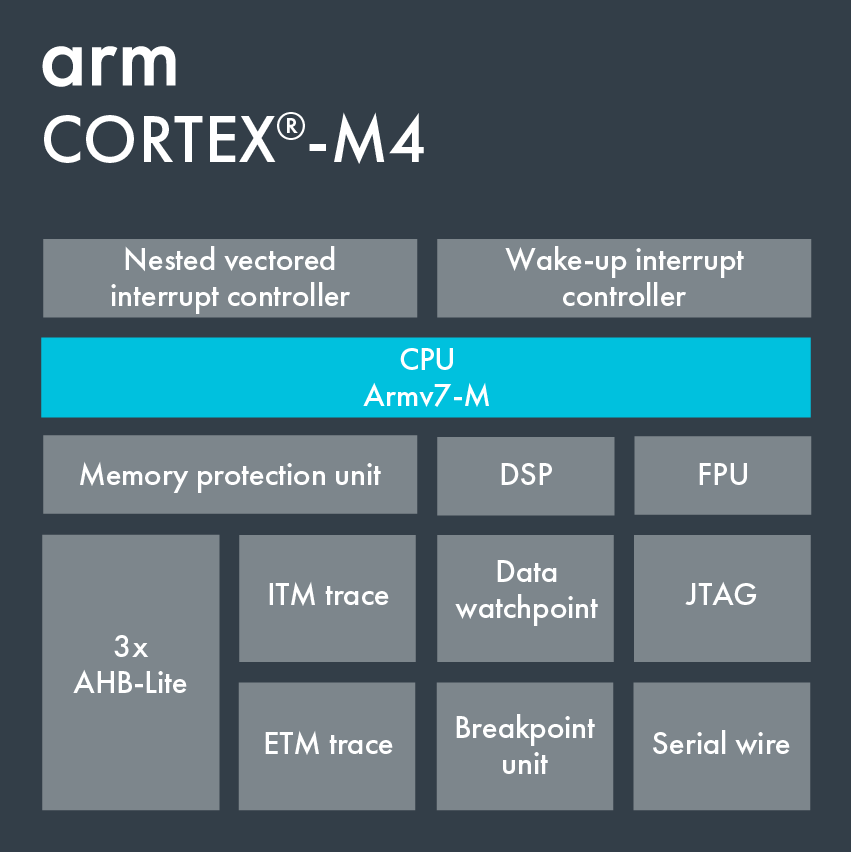
\includegraphics[width=.8\textwidth]{./Figures/Cortex-M4.png}
    \caption{Diagrama de la arquitectura \emph{Cortex M4}\citep{WEBSITE:cortexm}.}
	\label{fig:cortexm}
\end{figure}

\begin{figure}[htbp]
	\centering
	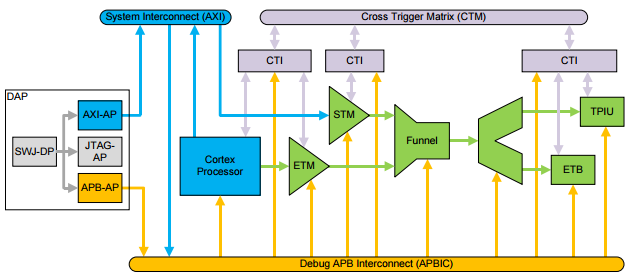
\includegraphics[width=\textwidth]{./Figures/coresight.png}
    \caption{Diagrama del módulo \emph{CoreSight}\citep{WEBSITE:coresight}.}
	\label{fig:coresight}
\end{figure}

\section{Servidores y sondas de depuración}
\label{sec:depuracion}

\begin{figure}[htbp]
	\centering
	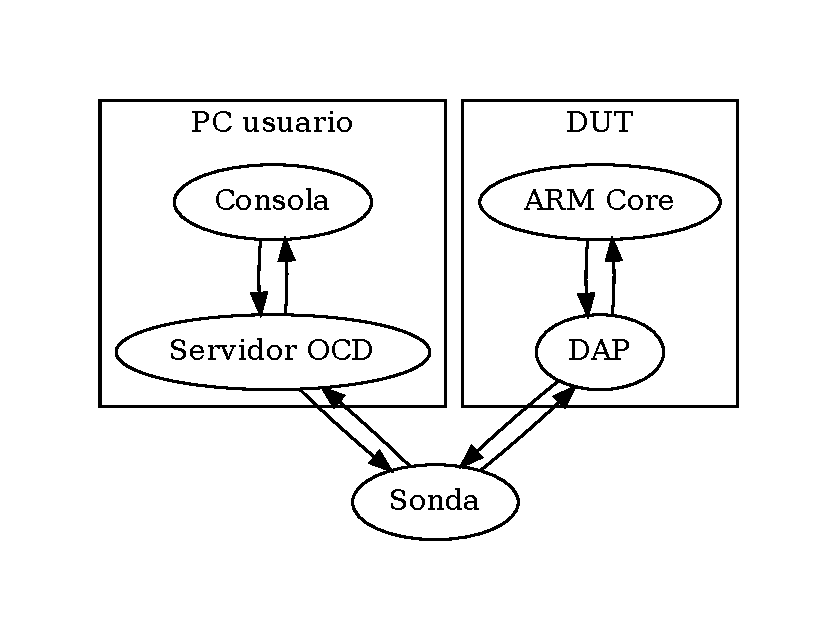
\includegraphics[width=.8\textwidth]{./Figures/debug.pdf}
    \caption{Conexión de una sesión de depuración.}
	\label{fig:debug}
\end{figure}

\begin{figure}[htbp]
	\centering
	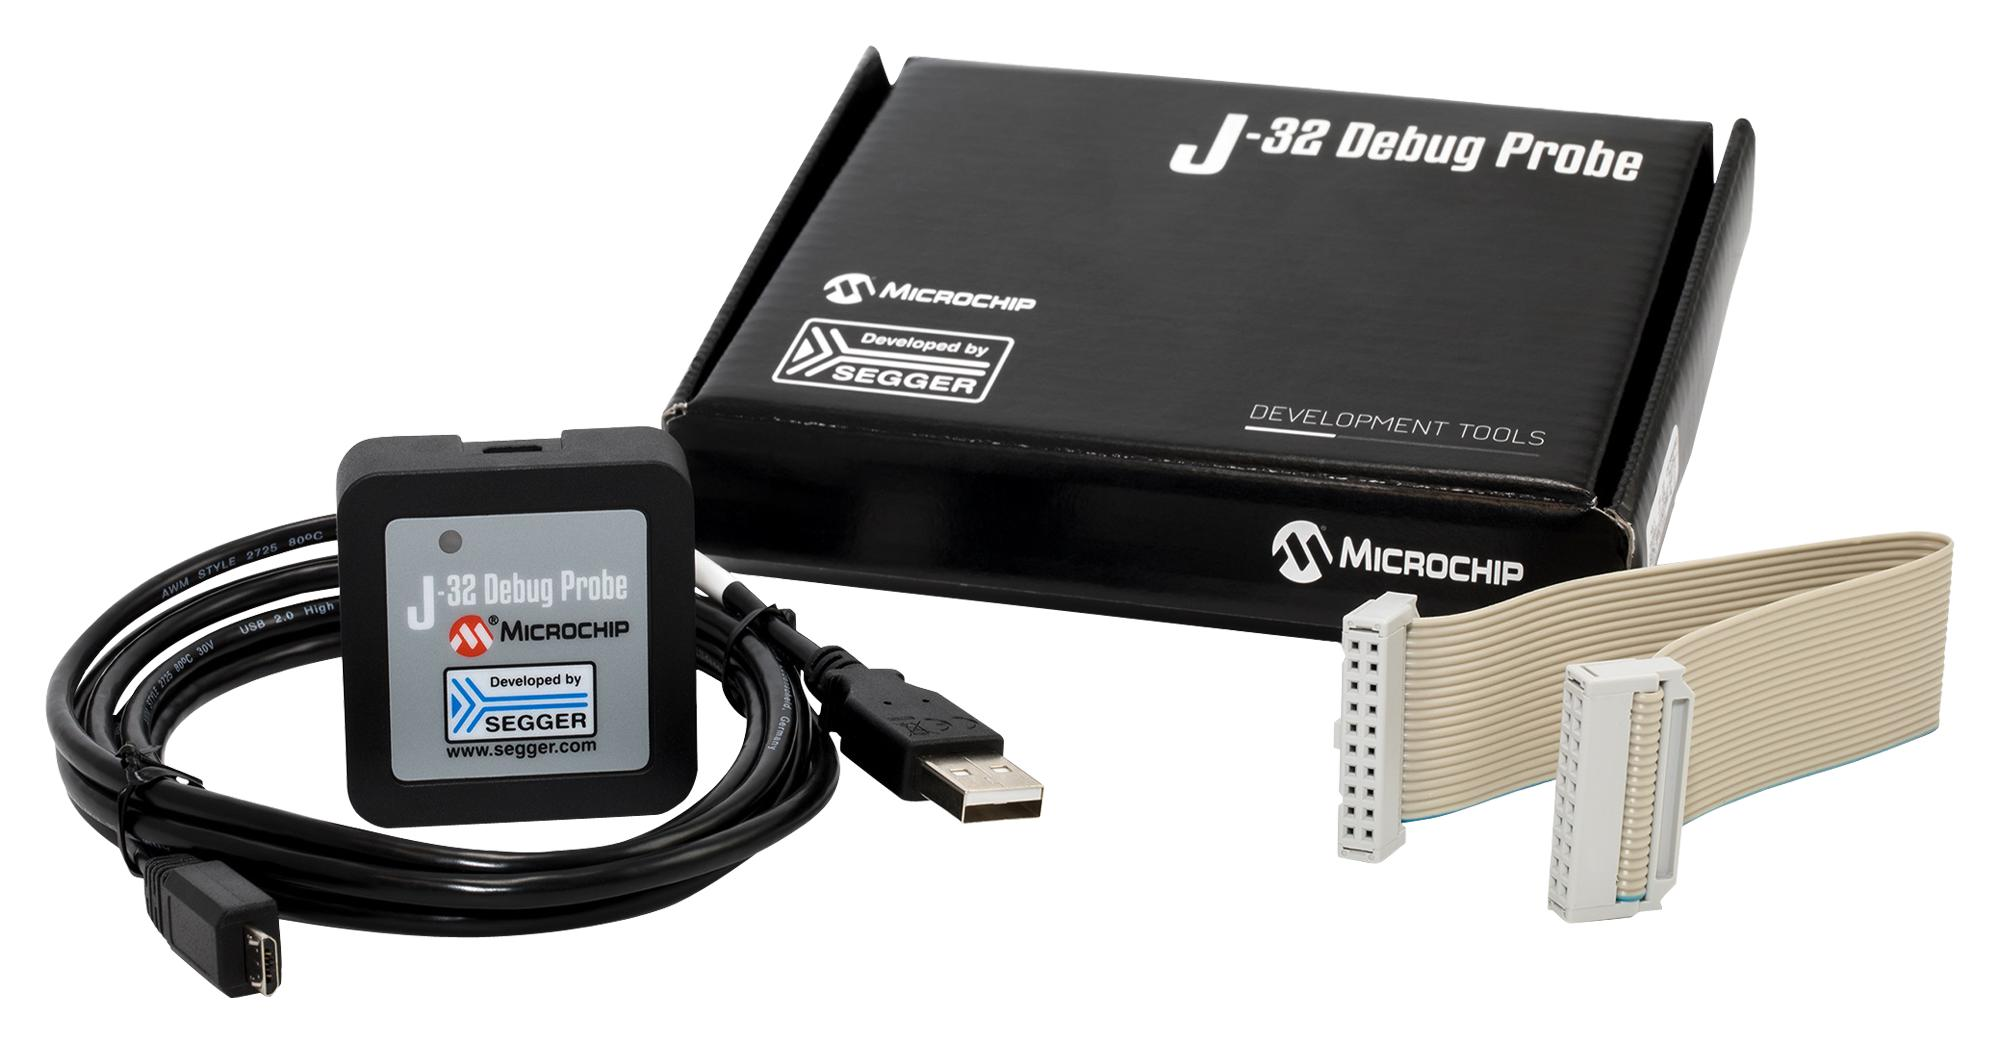
\includegraphics[width=.8\textwidth]{./Figures/segger.jpg}
    \caption{Sonda de depuración \emph{Segger J-32}.}
	\label{fig:sonda}
\end{figure}


% Tabla comparativa de servidores de depuración

\begin{table}[h]
	\centering
	\caption[Servidores de depuración]{Comparativa entre servidores de depuración}
	\begin{tabular}{l c c c}    
		\toprule
        \textbf{Servidor} & \textbf{API} & \textbf{Acceso}   & \textbf{Licencia}\\
		\midrule
        OpenOCD           & tcl                         & Registros y SDRAM & MIT\\        	
        PyOCD             & Python 3                    & Registros y SDRAM & Apache-2.0\\
		\bottomrule
		\hline
	\end{tabular}
	\label{tab:servidores}
\end{table}

\section{Periféricos de interés}
\label{sec:perifericos}

\begin{table}[h]
	\centering
	\caption[Resumen de periféricos]{Resumen de periféricos}
	\begin{tabular}{l c c}    
		\toprule
        \textbf{Periférico} & \textbf{Funcionalidad}\\
		\midrule
		CAN                 & Bus de comunicación de grado industrial\\        	
		PIO                 & Entradas y salidas digitales\\
		SPI                 & Interfaz de comunicación sincrónica\\
		UART                & Puerto para dispositivos serie\\
		Watchdog            & Detección de errores y reinicio del integrado\\
		\bottomrule
		\hline
	\end{tabular}
	\label{tab:perifericosresumen}
\end{table}

\section{Requerimientos del cliente}
\label{sec:emphuerimientos}

El software aquí especificado brindará las siguientes funcionalidades:

\begin{enumerate}
	\item Referentes al CCI:
		\begin{enumerate}
			\item Generará de una interfaz de usuario.
			\item Permitirá configurar el ensayo a realizar.
			\item Activará el Proceso de DUT.
			\item Observará la salida del DUT.
			\item Inyectará SEFI-SEU en el DUT.
			\item Persistirá las operaciones, entradas y salidas.
			\item Generará informes del ensayo realizado.
		\end{enumerate}
	\item Referentes al Proceso de DUT:
		\begin{enumerate}
			\item Verificará el estado de los periféricos del DUT.
			\item Detectará si el DUT perdió su secuencia.
			\item Generará reportes de estado de periféricos y secuencia.
			\item Permitirá que CCI configure el alcance de la secuencia.
			\item Permitirá que CCI maneje el flujo de su secuencia.
		\end{enumerate}
\end{enumerate}

Las restricciones del desarrollo del sistema son las siguientes:

\begin{itemize}
	\item Utilización de repositorio con control de versiones \emph{Gitlab}.
	\item Documentación del código con \emph{Doxygen}.
	\item Utilización exclusiva del lenguaje de programación \emph{Python 3}.
\end{itemize}

Los requerimientos de las interfaces externas son las siguientes:

\begin{enumerate}
	\item CCI:
		\begin{enumerate}
			\item Módulo para el usuario:
				\begin{itemize}
					\item \emph{001} deberá representar todos los caracteres de ISO Std. 10646.
					\item \emph{002} cumplirá con las secuencias de escape especificadas en ISO Std. 6429.
					\item \emph{003} usará el castellano como idioma conforme a la Real Academia Española.
					\item \emph{004} se aceptarán barbarismos que conformen la interfaz con los sistemas UNIX.
					\item \emph{005} no deberá producir destellos ni cambios bruscos en su intensidad lumínica.
					\item \emph{006} no deberá producir sonidos
					\item Títulos:
						\begin{itemize}
							\item \emph{007} los títulos deberán tener una longitud máxima de 30 caracteres.
							\item \emph{008} los títulos deberán estar correctamente capitalizados.
							\item \emph{009} los títulos deberán ser únicos.
						\end{itemize}
					\item Comandos:
						\begin{itemize}
							\item \emph{010} el sistema se iniciará con el comando \texttt{sise.py}.
							\item \emph{011} el sistema imprimirá en pantalla un manual de ayuda con el comando \texttt{sise --help}.
							\item \emph{012} se podrá exportar la configuración del último ensayo realizado con el comando \texttt{sise --export=Ruta}.
							\item \emph{013} se podrá importar la configuración de un ensayo a realizar con el comando \texttt{sise --import=Ruta/Archivo}.
						\end{itemize}
					\item Menú:
						\begin{itemize}
							\item \emph{014} el sistema de menú tendrá una arquitectura de árbol.
							\item \emph{015} la navegación entre los nodos del menú será consistente en todo el árbol.
							\item \emph{016} se indicará en todo momento el nodo actual y todos los nodos que lleven a la raíz del árbol.
						\end{itemize}
				\end{itemize}
			\item Con DUT:
				\begin{itemize}
					\item \emph{017} la comunicación con UART será en 9600 baudios, 8 bits de datos, 1 bit de parada y 0 bits de paridad.
					\item \emph{018} la comunicación con el debugger conformará con la configuración recomendada por el fabricante.
				\end{itemize}
		\end{enumerate}
	\item Proceso de DUT:
		\begin{itemize}
			\item \emph{019} la comunicación con el debugger estará disponible durante todo el flujo de la secuencia.
			\item \emph{020} durante el flujo de la secuencia, la UART solo podrá transmitir información.
			\item \emph{021} en el periodo entre secuencias, la UART podrá recibir y transmitir información.
		\end{itemize}
\end{enumerate}

Las funciones deben cumplir lo siguiente:

\begin{enumerate}
	\item CCI:
		\begin{itemize}
			\item \emph{022} detendrá la secuencia de duración $ T $ del DUT en un momento $ t $ definido como $ t \, \epsilon \, \rm I\!R^+ \wedge t \, < T$.
			\item \emph{023} con la secuencia del DUT detenida, inyectará un SEFI-SEU que invertirá el valor de un bit de un registro interno.
			\item \emph{024} La descripción del ensayo definirá el momento $ t $ de inyección de SEFI-SEU durante la secuencia de duración $ T $ y será un múltiplo de $\Delta t$ definido como $ \Delta t=T/N \, \forall \, N \epsilon \, \rm I\!N $.
			\item \emph{025} La descripción del ensayo definirá la cantidad $ M $ de registros involucrados en la prueba.
			\item \emph{026} La cantidad de secuencias $ L $ a ejecutar quedará definida como \\$ L = N \times M $.
			\item \emph{027} Se ejecutará una secuencia de control sin inyección de SEFI-SEU antes de correr las $ L $ secuencias.
			\item \emph{028} Por cada ejecución de una secuencia se obtendrá un valor de salida $ S $ del DUT.
			\item \emph{030} Cada valor de salida $ S $ será persistido para su análisis.
			\item \emph{031} Cada valor de salida $ S $ quedará asociado a su correspondiente secuencia con su inyección de SEFI-SEU y momento $ t $.
			\item \emph{032} Se generará un archivo de resultados llamado\\ \texttt{resultados-AAAAMMDDHHmm.res}, siendo AAAA el año del ensayo, MM el mes, DD el día, HH la hora y mm los minutos.
			\item \emph{033} El archivo de resultados acumulará los SEFI y SEU de cada registro del DUT.
			\item \emph{034} El archivo de resultados acumulará los SEU de cada periférico del DUT.
			\item \emph{035} El archivo de resultados indicará el FOM del registro definido como:
			$ FOM_{REG} = (1 - \frac{SEU}{SEFI}) $
			\item \emph{036} El archivo de resultados indicará el FOM del DUT definido como:
			$ FOM_{DUT} = \frac{1}{M} \times \sum_{i = 1}^{i = M}FOM_{i} $ siendo $ i $ el número que representa un registro del DUT.
			\item \emph{037} Se generará un archivo de histogramas llamado \\ \texttt{histogramas-AAAAMMDDHHmm.his} siendo AAAA el año del ensayo, MM el mes, DD el día, HH la hora y mm los minutos.
			\item \emph{038} El archivo de histogramas tendrá una tabla que indique la frecuencia de fallos como función de los SEFIs por registro del DUT.
			\item \emph{039} El archivo de histogramas tendrá una tabla que indique la frecuencia de fallos como función de los SEFIs por periférico del DUT.
		\end{itemize}
	\item Proceso de DUT:
		\begin{itemize}
			\item \emph{040} deberá correr una secuencia de autoevaluación cuya ejecución durará un tiempo $ T $.
			\item \emph{041} deberá producir una salida $ S $ que podrá ser un estado o una secuencia de estados.
			\item \emph{042} este proceso podrá tener una entrada $ E $.
			\item \emph{043} deberá evaluar el estado de los periféricos del DUT.
			\item \emph{044} tendrá una función de evaluación para cada uno de los periféricos del DUT.
			\item \emph{045} se podrá definir por la entrada $ E $ si se desea excluir uno o más periféricos en la secuencia.
			\item \emph{046} manejará una interrupción del flujo normal de la secuencia y generará una salida $ S $ indicando la excepción, por ejemplo: interrupción por \emph{watchdog}.
			\item \emph{047} la salida $ S $ utilizará la UART del DUT para ser transmitida.
			\item \emph{048} la entrada $ E $ utilizará la UART del DUT para ser recibida.
		\end{itemize}
\end{enumerate}

Requisitos de rendimiento:

\begin{itemize}
	\item \emph{049} la inyección de SEFI-SEU podrá tener un desvío en su momento $ t $ de 10 ms.
	\item \emph{050} el desvío tolerado de $ t $ deberá representar como máximo el 1\% de la duración $ T $ de la secuencia del DUT.
	\item \emph{051} aceptará un $ \Delta t $ que como mínimo represente el 5\% de la duración $ T $ de la secuencia del DUT.
\end{itemize}

Restricciones de diseño:

\begin{itemize}
	\item \emph{052} se utilizará como dispositivo principal el microcontrolador seleccionado por INVAP.
	\item \emph{053} se utilizará un sistema operativo de tiempo real para diseñar el Proceso de DUT.
\end{itemize}

Los atributos del sistema son los siguientes:

\begin{enumerate}
	\item Mantenibilidad:
	\begin{itemize}
		\item \emph{054} el Proceso de DUT se desarrollará con un modelo de capas.
	\end{itemize}
\end{enumerate}
